\documentclass{scrartcl}


\title{Forschungsarbeit}
\author{Laura Schillke, Sebastian Meidel, Mekong Lam }
\date{October 2018}

% Pakete laden 

\usepackage{graphicx}
\usepackage[utf8]{inputenc}
\usepackage[T1]{fontenc}
\usepackage[german]{babel}
\usepackage[default,osfigures,scale=0.95]{opensans}  %% Option 'sfdefault' only if the base font of the document is to be sans serif
% Verlinke Zitate
\usepackage{hyperref}
% Verlinke das Inhaltsverzeichnis
\hypersetup{linktocpage}
\usepackage{csquotes}
\usepackage[style=authortitle-dw,
idembib=false,
idemtracker=false,
backend=biber
]{biblatex}
\usepackage{graphicx}
\addbibresource{mendeley_v3.bib}
%----------------------------

%----------------------------

%Dokument beginnt
\begin{document}

\maketitle


\newpage

\setcounter{tocdepth}{3}
\tableofcontents 



\newpage

\section{Zusammenfassung}
Bacon ipsum dolor amet shank biltong t-bone ham, ground round pastrami boudin porchetta cow fatback turkey pork tenderloin salami. Buffalo meatloaf ham hock alcatra. Boudin ground round chicken porchetta ham. T-bone spare ribs chuck fatback.

\section{Einleitung}
Bacon ipsum dolor amet shank biltong t-bone ham, ground round pastrami boudin porchetta cow fatback turkey pork tenderloin salami. Buffalo meatloaf ham hock alcatra. Boudin ground round chicken porchetta ham. T-bone spare ribs chuck fatback.

%\begin{figure}[h!]
%\centering
%
\includegraphics[scale=1.7]{universe}
%\caption{The Universe}
%\label{fig:universe}
%\end{figure}

\section{Definitionen}

\subsection{Stadt}

Haas und Neumair zufolge bezeichnet man eine Stadt als eine größere verdichtete Siedlung, die mit bestimmten Funktionen und Merkmalen charakterisiert wird \footcite{HaasDefinitionWirtschaftslexikon}. Die Definition des Brockhaus schreibt einer Stadt Merkmale zu wie zum Beispiel die eigene Versorgungs- und Verwaltungsstruktur, die innere Gliederung oder eine höhere Bebauungs- und Verkehrsdichte. Hinzu kommen spezielle Funktionen wie politische Aufgaben (Haupstädte, Festungsstädte) oder wirtschaftliche Funktionen (Hansestädte, Hafenstädte, Karawanenstädte). \footcite{BrockhausStadt} Die statistischen Kriterien, die eine „Stadt“ vom „Land“ unterscheiden variieren von Land zu Land. Beispielsweise werden Städte in der Bundesrepublik Deutschland mit 
\begin{itemize}
\item 5.000 bis 20.000 Einwohnern als „Kleinstadt“,
\item 20.000 bis 50.000 Einwohnern als „Mittelstadt“,
\item ab 100.000 Einwohnern als „Großstadt“ 
\end{itemize}
bezeichnet \footcite{Institutinternationaldestatistique1887BulletinStatistique}. Demgegenüber orientiert man sich in China an die Bevölkerungsdichte: 

\begin{displayquote}
In the case of cities with district establishment, the city proper refers to the whole administrative area of the district if its population density is 1 500 people per kilometre or higher [...]. \footcite[S.~2]{UnitedNations2005Table2005} 
\end{displayquote}

Unabhängig von regional unterschiedlichen Kriterien lässt sich mit steigender Einwohnerzahl und -dichte einer Stadt folgern, dass auch die Anforderungen an gewährleisteter Lebensmittelversorgung für die städtische Bevölkerung steigen. D.h. die Lebensmittelversorgung einer Großstadt zu gewährleisten ist schwieriger als die einer Kleinstadt. Noch größer ist die Herausforderung in Megastädten. Den Vereinten Nationen zufolge wird eine Megastadt (englisch: „Megacity“) als eine Stadt bezeichnet mit mindestens 10 Millionen Einwohnern. Im Jahr 2016 existierten 31 Megastädte und Prognosen zufolge steige die Anzahl der Megastädte im Jahr 2030 auf 41 \footcite{UnitedNations2016The2016}. Tokio zählt mit 38 Millionen Einwohnern als die größte Megastadt weltweit und derzeit befinden sich die meisten Megastädte in Industrie- und Entwicklungsländern (wie in Abbildung \ref{figUrban} erkennbar). 

\begin{figure}[h]
\centering
\hspace*{-4cm}   
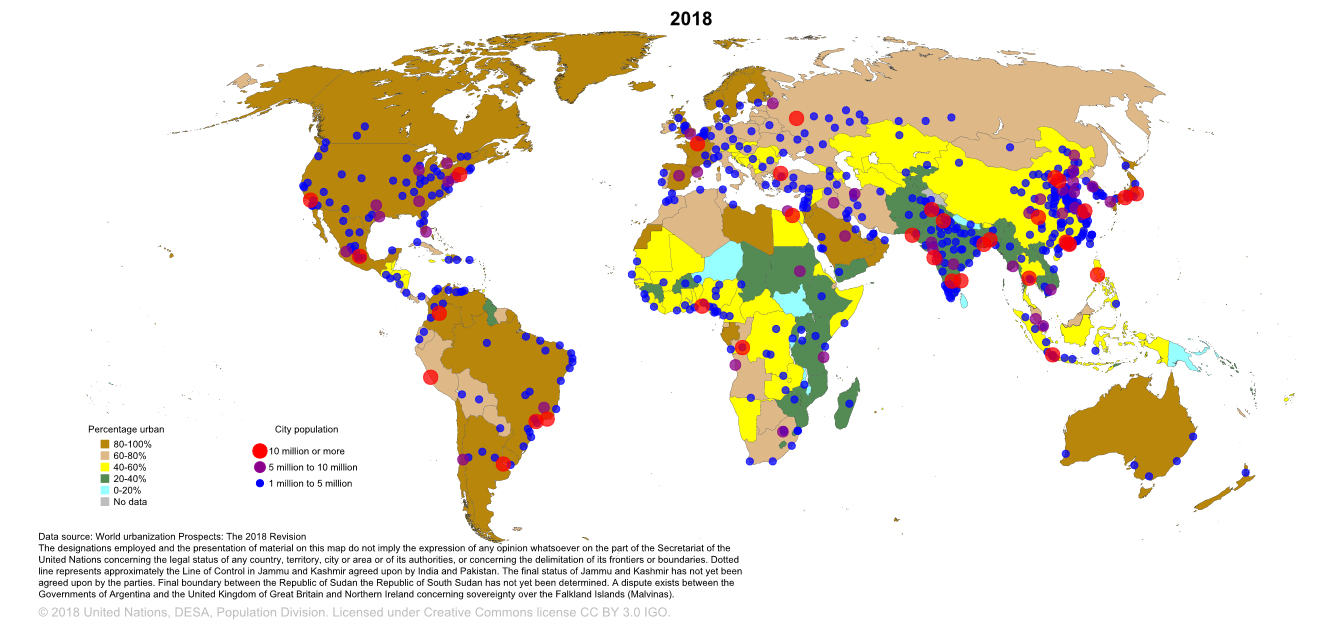
\includegraphics[width=20cm]{image_folder/CityPop_Urban.png}
\caption{Urbanisierung der Welt}
\label{figUrban}
\end{figure}

In der obigen Abbildung erkennt man, dass Nord- und Südamerika sowie Europa deutlich verstädtert sind, wohingegen viele Regionen in Afrika und Asien mehr ländliche Gebiete beinhalten. In dieser Forschungsarbeit wird der Stadtbegriff im Bezug zu ihrer fähigen Lebensmittelversorgung und Nachhaltigkeit betrachtet. Daher eignet es sich Städte im Unterschied zu ländlichen Gemeinden zu beschreiben: 

\begin{displayquote} 
„The hallmarks of cities are: (a) a large population that (b) aggregates in a central location with (c) buildings and monuments that (d) represent institutions that organize and facilitate productivity.“ \footcite[S.16]{Elmqvist2013}. 
\end{displayquote}  Zusammenfassend heißt es, dass Städte sich kennzeichnen lassen durch eine große Einwohnerzahl angehäuft an einem zentralen Ort mit Bauten und Monumenten, die Institutionen repräsentieren und produktive Leistungen organisieren und ermöglichen.

\subsubsection{Stadtökosysteme}
Stadtökosysteme sind Ökosysteme, die von Menschen erzeugt und beeinflusst werden. Wesentliche Merkmale eines Stadtökosystems sind der hohe Anteil an bebauter und versiegelter Fläche und eine hohe Bevölkerungsdichte. Genauer gesagt führt diese hohe Dichte an verschiedenen Landnutzungen dazu, dass natürlichen Ressourcen wie Wasser, Luft, Boden und Biodiversität extrem beansprucht werden. Desweiteren lässt sich über Stadtökosysteme sagen, dass ihr Erhalt von der externen Einfuhr an Lebensmitteln und Ressourcen abhängig ist  \footcite[S.61]{Breuste2016Stadtokosysteme}.


\subsection{Nachhaltigkeit}

Der Begriff Nachhaltigkeit ansich ist ein vielschichtiger Begriff. Er findet Verwendung in der Wirtschaft, Ökonomie, Ethik und Ökologie. Nachhaltigkeit kann als Art und Weise des Wirtschaftens bezeichnet werden, „bei welcher derzeitige Bedürfnisse befriedigt werden, ohne zukünftigen Generationen die Lebensgrundlagen zu entziehen. \footcite{DefinitionWirtschaftslexikonb}. Ebenso kann der Begriff als Brücke zwischen ökologischen und ökonomischen Interessen gesehen werden. Seinen Ursprung hat das Prinzip der Nachhaltigkeit in der Forstwirtschaft des 18. Jahrhunderts. Nach einer Übernutzung der Wälder und daraus resultierend knapper werdenden Holzbeständen, wurde mit Nachhaltigkeit ein Bewirtschaftungsprinzip gefordert, bei dem regenerativ gearbeitet werden sollte, das heißt “nicht mehr Holz geschlagen werden als nachwächst.“ \footcite{NachhaltigeBrockhaus.de}
Ab dem 19. Jahrhundert wurde zu dieser rein ressourcenökonomischen Betrachtungsweise von Nachhaltigkeit eine Umfassendere hinzugefügt, die sämtliche Funktionen des Waldes in Betracht zieht.

\hfill \break
Der Begriff Nachhaltigkeit kann in stark und schwach eingeteilt werden.\footcite{Nachhaltigkeit}


\begin{itemize}
\item die starke Nachhaltigkeitstellt die Erhaltung der natürlichen Ressourcen in den Vordergrund. Sie beruht auf der Annahme, dass Naturgut nicht durch andere Kapitalformen ersetzt werden kann,
\item schwache Nachhaltigkeit beruht auf der Annahme das Kapital- oder Naturgut durch andere Kapitalformen erstetzt werden kann.
\end{itemize}
Konfliktpotenzial zwischen den Vertretern jeweiliger Positionen treten vor allem bei der Frage auf, "wie heute verursachte, aber zukünftig auftretende Umweltschäden beziehungsweise Ressourcenknappheiten zu bewerten sind.\footcite{NachhaltigeBrockhaus.de}



\subsubsection{Nachhaltige Entwicklung}
  Ziel der Nachhaltigen Entwicklung ist eine dauerhalfte und gerechten Bewirtschaftung der Erde.\footcite{NachhaltigeBrockhaus.de} Die Bezeichnung wurde vom Begriff der Nachhaltigkeit abgeleitet. In der Agrar- und Ernährungswirtschaft definiert der Begriff eine "dauerhafte Nutzung von Ressourcen bei gleichbleibender bzw. wachsender Effektivität". \footcite{oppenhauser2010nachhaltigkeit} Im internationale Sprachraum hat sich der Begriff "Sustainable Development" als Definition gefestigt. In der internationalen Politik und bei gesellschaftlichen Bewegungen wird die Nachhaltige Entwicklung als Leitbild eingesetzt.\footcite{oppenhauser2010nachhaltigkeit}
 
 Konkrete Umsetzungsmethoden von Nachhaltiger Entwicklung stellen in Entwicklungsländern hauptsächlich Entwicklungsaspekte in den Vordergrund, in den industrialisierten Ländern geht es um den langfristigen Schutz und Erhalt der natürlichen Lebensgrundlage. 



\subsubsection{Ökologische Nachhaltigkeit}
„Die ökologische Nachhaltigkeit bezieht sich allgemein auf das Überleben und den Gesundheitszustand von Ökosystemen.“ \footcite{DefinitionWirtschaftslexikonc}  Sie bezeichnet einen weitsichtiger und rücksichtsvoller Umgang mit natürlichen Ressourcen. Sofern die ökologische Nachhaltigkeit vernachlässigt wird, kann dies dazu führen, dass bestimmte Ressourcen unbrauchbar oder unwiderruflich zerstört werden, was jegliche weitere Entwicklungen der Ressource und ihrer Umgebung unmöglich machen kann. Laut Berding und Bukow in "Die kompakte Stadt der Zukunft - Auf dem Weg zu einer inklusiven und nachhaltigen Stadtgesellschaft (s.95) \footcite{BerdingWolf-DietrichBukowKarinCudakHrsgDieStadtgesellschaft} gewinnt das Thema Nachhaltigkeit für die Stadtentwicklung an neuer Wichtigkeit. 



\subsubsection{Ökosystem}
Als Ökosystem bezeichnet man ein Wirkungsgefüge von Arten und ihrem Lebensraum. Es besteht aus Produzenten und Destruenten. Dazwischen befindet sich eine Reihe an Konsumenten. Vereinfacht dargestellt entsteht auf diese Weise eine Nahrungskette. Dieses Nebeneinander auf kleistem Raum aus Pflanzen und Tieren befindet sich stets in einem zyklischen Prozess. Je enger die Nahrungsketten ineinander verwoben sind und je artenreicher das Wirkungsgefüge ist desto komplexer ist das Ökosystem.\footcite{NachhaltigeBrockhaus.de} Die Agrarlandschaft kann als ein vom Menschen stark beeinflusstes und künstliches Ökosystem angesehen werden. vgl.\footcite{BrockhausOkosystem}
Ökosysteme sind offene Systeme, die einseitig von der Sonne Energie aufnehmen. Die Stoffkreisläufe inerhalb des Systems sind unter optimalen Umständen ausgeglichen. Es entsteht ein dynamisches Gleichgewicht. \footcite{BrockhausOkosystem}

\hfill \break
Stabilität und Gefährdung: Komplexe Ökosysteme sind stabiler als einfache Ökosysteme, gleichzeitig sind diese schwerer oder unmöglich regenerierbar, während einfache Ökosysteme sich und ihr Gleichgewicht einfach wiederherstellen können. Als Beispiel kann der Vergleich zwischen einem einfachem Ökosystem (Nadelwald) und einem komplexem Ökosystem (Regenwald) herangezogen werden.
In einem einfachen System kann der Verlust oder die Veränderung einzelner Komponenten (Überdüngung, Wasserknappheit oder Überwässerung in Brachregionen) das eigene Gleichgewicht sowie das Gleichgewicht angrenzender Ökosysteme schneller in Gefahr bringen. \footcite{DefinitionWirtschaftslexikone}

\begin{figure}[htp]
\centering
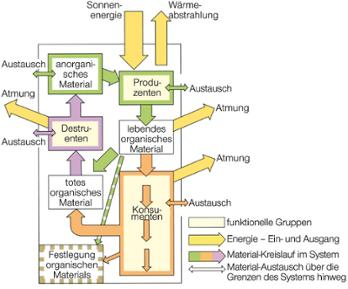
\includegraphics[width=5cm]{image_folder/oekosystemkreisslauf.png}
\caption{Ökosystemkreisslauf: Kreislauf: Verknüpfung von Konsumenten Destruenten und Produzenten}
\label{fig:Ökosystemkreisslauf}
\end{figure}
        
\subsubsection{Ökoeffizienz}
Ökoeffizienz wird als das Verhältnis von ökologischer Schadschöpfung einer Tätigkeit oder eines Produkts zu seiner ökonomischer Wertschöpfung beschrieben.\footcite{ vgl. Schaltegger1990OkologischeUnternehmung} 

\begin{figure}[h]
\centering
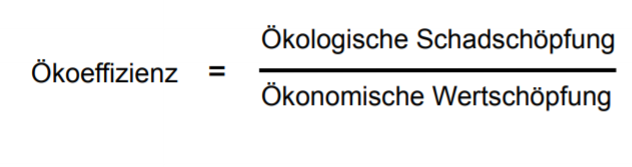
\includegraphics[width=5cm]{image_folder/oekoeffizienz.png}
\caption{Ökoeffizienzgleichung}
\label{fig:Ökoeffizienzgleichung}
\end{figure}\footcite{Essel2010AnalyseFazit}

   
 Der WBCSD\footnote{ein Zusammenschluss international tätiger Unternehmen, der das Ziel hat, Wirtschaftswachstum und Nachhaltigkeit in Einklang zu bringen} hat "für Ökoeffizienz folgende Kriterien erstellt: 
 
 \begin{itemize}
 \item die Bereitstellung wettbewerbsfähiger Produkte
 \item die Befriedigung menschlicher Bedürfnisse 
 \item die Förderung der Lebensqualität
 \item die Minimierung der Umweltauswirkungen und Ressourcenintensität während des gesamten Produktlebens\footcite{OkoeffizienzBrockhaus.de}
 \end{itemize}

Als Ökoeffizient werden Strategien und Konzepte bezeichnet, die sich dazu eignen nachhaltige Produktionsmethoden umzusetzen. Die Kriterien sind laut WBCSD folgende:
\begin{itemize}
\item geringer Einsatz natürlicher Ressourcen
\item geringe Umweltbelastung
\item zu ersteren beiden im Vergleich hoher Ertrag
\end{itemize}


Ökoeffizienz kann u.a. erreicht werden durch:
\begin{itemize}
\item Minimierung des Material- und Energieverbrauchs pro Produktmenge,
\item Verwendung recyclingfähiger Materialien,
\item Einsatz erneuerbarer Ressourcen, Vermeidung des Einsatzes toxischer Substanzen,
\item Erhöhung der Lebensdauer beziehungsweise des Nutzens eines Produktes.
\end{itemize}

Methodische Ansätze zur Messung der Ökoeffizienz von Produkten sind:
\begin{itemize}
\item Stoffstrommanagement
\item die Umweltbilanz
\item Ökoeffizienz-Analyse Bewertungsmethode der BASF \footnote{Sie entstand 1995 und bewertet die Wirtschaftlichkeit eines Produkts im Verhältnis zu seiner Umweltbelastung. Betrachtet wird der Produktlebensweg beginnend bei der Rohstoffgewinnung über die Herstellung und Verwendung bis zur Entsorgung.}
\end{itemize}
\footcite{DefinitionWirtschaftslexikonc} (Quelle des gesamten Abschnitts)

\subsubsection{Bewertung von Nachhaltigkeit}
Es gibt eine Vielzahl an Werkzeugen zur Bewertung von Nachhaltigkeit. Sie unterscheiden sich je nach Zielsetzung und Fokus. Im Folgenden werden die für diese Forschungsarbeit relevantesten Methoden vorgestellt: 

\begin{itemize}
\itemÖkoeffizienz-Analyse und SEEBALANCE®
\item GEMIS-Projekte
\item IINAS: Entwicklung eines globalen Nachhaltigkeitsstandards zur Landnutzung (GLOBALANDS)
\item Nachhaltigkeitsstrategien
\end{itemize}

\subsubsection{Bewertung von Nachhaltiger Landnutzung}
Das Framework for Evaluating Sustainable Land Management FESLM von Smyth & Dumanski wurde in den 90er Jahren von der FAO (Food and Agriculture Organisation) entwickelt und von Drechsel et al. (2008) erweitert.
\begin{figure}[h]
\centering
\includegraphics[width=5cm]{image_folder/drechel.png}
\caption{Bewertung von Nachhaltiger Landnutzung}
\label{fig:Bewertung von Nachhaltiger Landnutzung}
\end{figure}\footcite{TobiasSpringDerBasel-Stadt, S.17}

\subsubsection{ökologischer Fußabdruck}

“Die (Natur-)Fläche, die zur Aufrechterhaltung der Energie- und Materialflüsse einer Wirtschaftseinheit wie z. B. einer Stadt benötigt wird, ist deren ökologischer Fußabdruck. Er ist ein Werkzeug zur Bilanzierung des menschlichen Naturverbrauchs und wird in globalen Hektaren angegeben.„Der ökologische Fußabdruck misst so die‚ ökologische Tragfähigkeit’ einer Bevölkerung“ (Wackernagel & Rees 1997: 25).” \footcite{MichelsenGrundlagenEntwicklung, S.5}. 
(vgl.) MathisWackernagelUnserNimmt, S. 23–25)
"Die Inanspruchnahme von Ressourcen einer Person, einer Stadt oder eines Landes"\footcite{AntjeFlade2015StadtStadtforschung, S.192} können somit anhand des ökologischer Fußabdruck verglichen werden. 

\begin{displayquote}
“Der ökologische Fußabdruck von London – als Beispiel für eine Großstadt in einem hoch entwickelten Land – ist z. B. um etwa das Dreihundertfache größer als die Stadtfläche von London (Wackernagel et al. 2006), und damit wird deutlich, dass die Bevölkerung Londons auf ein Vielfaches der Stadtfläche – nicht nur im Umland, sondern weltweit – angewiesen ist. Da die globale Menge an Biokapazität begrenzt ist, veranschaulicht der ÖF ebenso das bestehende Ungleichgewicht.”\footcite{AntjeFlade2015StadtStadtforschung, S.192}
\end{displayquote} 

Durch die Berechnung dieses Fußabdrucks kann also nachvollzogen werden ob ein jeweiliger Konsum nachhaltig ist oder nicht.\footnote{AntjeFlade2015StadtStadtforschung, S.192 }



\subsubsection{Konfliktpotenziale bei der Umsetzung und Bewertung von Nachhaltiger Entwicklung}

Bei der Frage wie nachhaltige Entwicklung effizient und lösungsorientiert umgesetzt werden solle, stellen sich neben der Frage nach der Verantwortlichkeit für die Verursachung der Umweltprobleme und die Gerechtigkeitfrage nach der Verteilung der endlichen Ressourcen ("Global commons"). 

Nach dem Rio-Abkommen aus dem Jahr 1992 wurde diese Frage "von zahlreichen Kommentatoren so beantwortet, dass im Prinzip jeder Mensch weltweit das gleiche Recht hat, die globalen Gemeinschaftsgüter in nachhaltiger Weise zu nutzen. Dieser Interpretation wird entgegengehalten, dass sie regional unterschiedliche Bedürftigkeiten und kulturelle Besonderheiten ignoriere.” \footcite{NachhaltigeBrockhaus.de} Ebenso besteht der "Einwand, dass neben den unterschiedlichen Bedürftigkeiten auch das unterschiedliche Leistungsvermögen berücksichtigt werden müsse."\footcite{NachhaltigeBrockhaus.de} Demnach sei das zulässige Nutzungsniveau eines Staates nicht nach der Größe seiner Bevölkerung, sondern nach seinem Beitrag zur globalen Wertschöpfung zu bestimmen."\footcite{NachhaltigeBrockhaus.de}

\begin{figure}[h]
\centering
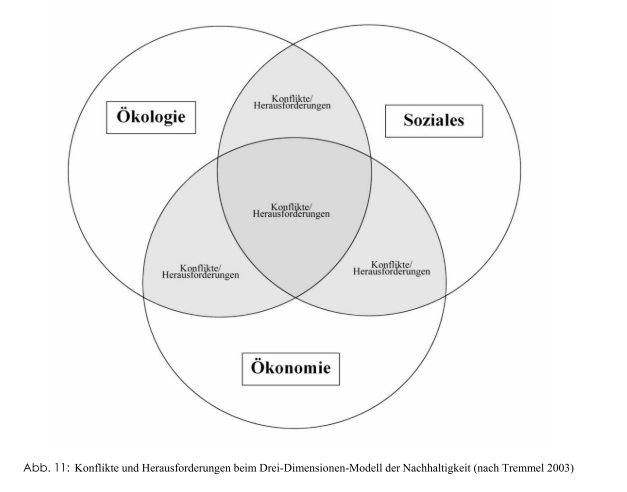
\includegraphics[width=10cm]{image_folder/dreidimensionenmodell_der_N.png}
\caption{3-dim-Modell}
\label{fig:3-dimensionen Modell}
\end{figure}

Konfliktpoltenzial besteht ebenfalls bei der Priorisierung von Lösungsvorschlägen. Eine Nachhaltige Lösung im sozialen Sinn kann auf Kosten von ökologischer Nachhaltigkeit gehen und umgekehrt. Genauso kann auch eine Win-Win Situation entstehen.

Länder des Südens stellen bislang die sozialen und ökonomischen Aspekte in den Vordergrund, Länder des Nordens wird dadurch die Hauptlast bei der Lösung der bestehenden Probleme im Ökologischen Bereich zugeschrieben. Die Länder des Nordens stellen ök. Apekt in den Vordergrund, nicht zuletzt weil sie es sich leisten können. SIe fordern gleichzeitig Lösungsinitative von Ländern des Südens.

\begin{figure}[h]
\centering
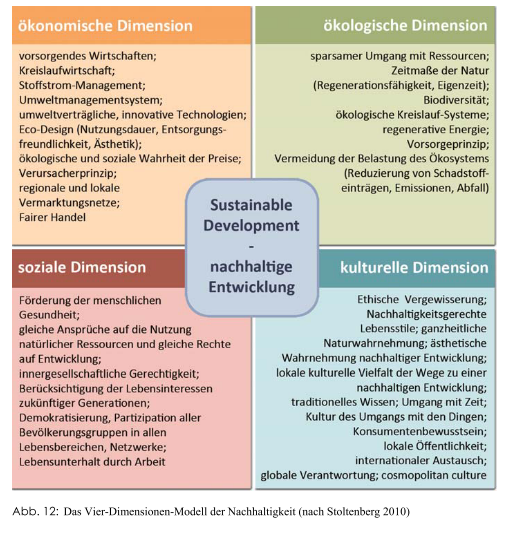
\includegraphics[width=6cm]{image_folder/vierdimensionenmodell_der_N.png}
\caption{4-dim-Modell}
\label{fig:4-dimensionen Modell}
\end{figure}

\subsubsection{Kritik am Begriff der nachhaltigen Entwicklung}\footcite{NachhaltigeBrockhaus.de}
Die übermäßige Verwendung des Begriff führt bei vielen Kritikern zu Misstrauen. Folgende Meinungen werden vertreten:

\begin{itemize}
\item Begriff sei überladen und als Sammelbegriff für alles Gute, was unerfüllbare Erwartungen wecke
\item Nachhaltige Entwicklung sei utopisch und eine Illusion
\item Beliebigkeit des Begriffs: “Unter der Flagge der nachhaltigen Entwicklung könne man trotzdem für komplett gegensätzliche Dinge eintreten.”
\item Meinung: Nachhaltigkeit sei inhaltslos und habe nur rhetorische FUnktionen, was die Leitbildfähigkeit des Begriffs außer Kraft setze
\end{itemize}

\subsubsection{Nachhaltigkeitswissenschaften}
Allgemein lässt sich festhalten, dass sich die "Nachhaltigkeitsforschung [...] mit Problemen, die die langfristige Sicherung der gesellschaftlichen Entwicklungsbedingungen gefährden" befasst.  \footcite{MichelsenGrundlagenEntwicklung, S.126}
Ihre Anfänge hatte die Nachhaltigkeitswissenschaft im Rahmen der Forschung zum Globalen Wandel in den späten 1980er Jahren. Laut der Autoren des..  gab unter anderem die Publikation „Die Grenzen des Wachstums“ von Meadows et al. 1972 den Anstoß zur Forschung bezüglich der Frage der globalen Umweltprobleme.
Drei internationale Großforschungsprogramme werden beüglich der Nachhaltigkeitswissenschaften insbesondere genannt: (1) das „International Geosphere-Biosphere Programme (IGBP)“, (2) das „World Climate Research Programme“ und (3) das
„International Research Programme on Biodiversity (DIVERSITAS)“.


\begin{figure}[htp]
\centering
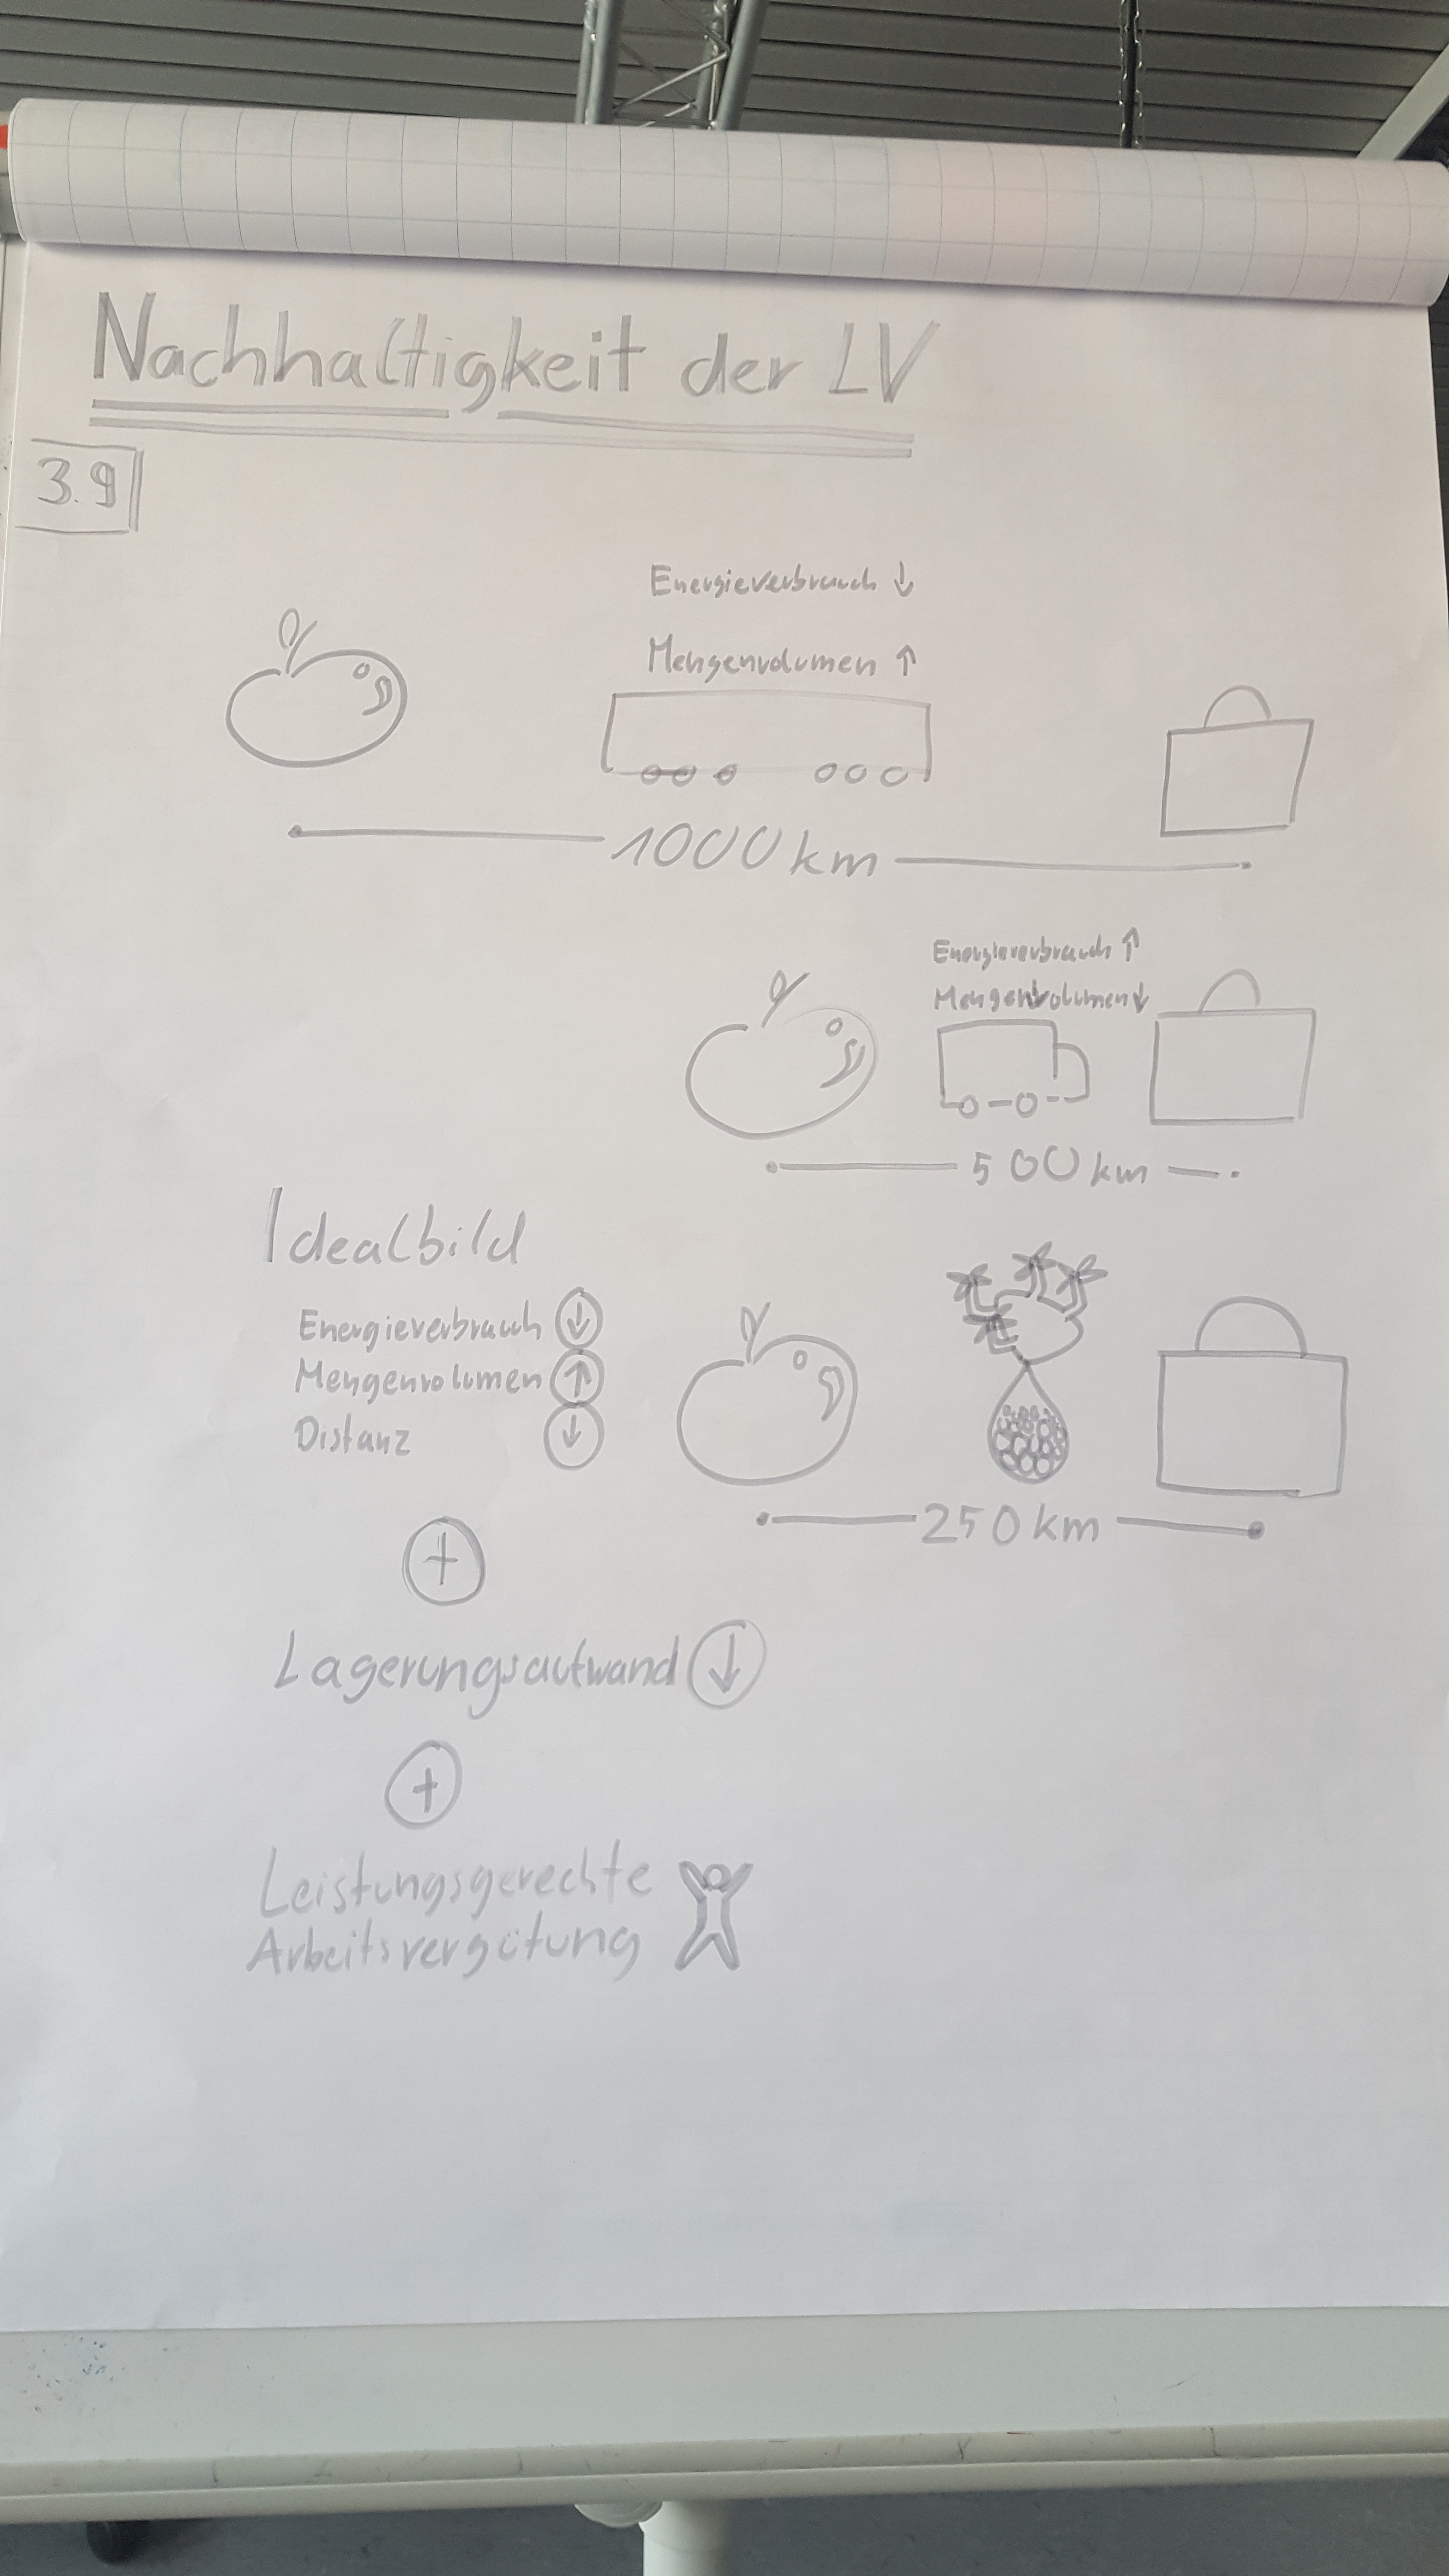
\includegraphics[width=5cm]{image_folder/skizze1.jpg}
\caption{Nachhaltigkeit der LV}
\label{fig:Skizze_Nachhaltigkeit}
\end{figure}

\section{Geschichte der Urbanisierung}

Wie Städte entstanden sind und sich bis heute ausbreiten hat viel damit zu tun wie Menschen das Problem der Nahrungsmittelsicherung lösten. Elmquist, Redman, Barthel und Costanza beschreiben in „Urbanization, Biodiversity and Ecosystem Services: Challenges and Opportunities“ hierzu drei vergangene Lösungsansätze, auf das sich dieses Kapitel überwiegend bezieht  \footcite[S.14ff]{Elmqvist2013}. 
\\
\\ 
Der erste Ansatz war das Nomadentum. Menschen zogen von Gegend zu Gegend, um sich zu ernähren. Sie folgten Tierherden sowie klimatisch günstigeren Regionen, wo nahrhafte Rohstoffe zu finden waren. Der zweite Ansatz war die Domestizierung von Tieren und Pflanzen. D.h. Rohstoffe wurden passend nach Bedarf herangezüchtet, geerntet und wieder angebaut. Menschen waren dadurch weniger von wechselnden Bedingungen ausgesetzt und verbesserten stetig ihre Nahrungsmittelerzeugung. Das erlaubte dauerhafte Sesshaftigkeit und förderte eine sichere Existenzgrundlage. Aus diesem Grund setzten sich kleine ländliche Gemeinden zur verbreitetesten Siedlungsform auf der Erde durch. Sie waren zwar unabhängig und isoliert voneinander, zeichneten sich allerdings als besonders widerstandsfähig gegenüber dem vorherigen Lebensstil aus. Für Elmquist et. al. war es also keine Überraschung, dass die Bevölkerungszahl dadurch anstieg. Darüber hinaus wuchsen ländliche Gemeinden derart, dass die Menge an Menschen überschüssig zur nötigen Arbeit auf dem Acker war. \\
\\
Den Höhepunkt dieses Prozesses bildete 5500 v.C. die erste städtische Siedlung in Mesopotamien - der dritte Ansatz. Die dortigen Innovationen wie das Schreiben, Monumentalbauten oder vertiefende Handwerkskünste zeigten das Potenzial dieser neuen Siedlungsform. Die Autoren bezeichnen Städte als Zentren der Innovation. Verglichen mit ländlichen Gemeinden zeichnet sich eine Stadt durch eine äußerst diverse und voneinander abhängige Gemeinschaft aus. Ländliche Gemeinden sind zwar unabhängiger und selbstversorgend, dafür war das Wachstum dieser Siedlungsform begrenzt. Anders verhält es sich mit Städten. Bezüglich der Versorgung war eine Stadt auf die umliegenden Gemeinden angewiesen. Jedoch trug der Austausch von Waren, technologische Erfindungen, Wissenschaft und Mathematik enorm zum Wachstum und der Verbreitung von Städten bei. Hinzu kam, dass eine soziale Erneuerung nötig war um diese große Gruppe von Menschen und groß skalierte produktive Aktivitäten zu organisieren. Eine klassenstrukturierte Gesellschaft, eine formalisierte Rechtsgrundlage und eine territoriumsbasierte Regierung bildeten daher den charakteristischen Rahmen. Damit eine Gemeinschaft auf diesen dichten Lebensraum funktionierte, war nämlich eine gewisse Ordnung im Miteinander nötig. Desweiteren waren Bauern in der Lage mehr Nahrungsmittel zu produzieren und zu lagern. Jedoch kam der Anreiz dazu erst durch die neue soziale Entwicklung mit Klassen, die sich mit haltbaren prestige Objekten identifizierten. 
\\
\\
Der wachsende Wohlstand in Städten führte zu regelmäßigen militärischen Angriffen. Zum Schutz wurden daher Stadtmauern gebaut. Diese städtebauliche Eingrenzung führte mit steigendem Wohlstand bei einer wachsenden Bevölkerung zu einem dichteren Stadtökosystem, das kennzeichnend für viele heutige Städte ist. Der nötige Anbau an Rohstoffen fand daher meistens im Umland statt, weswegen viele Dorfgemeinden nahe an Städte ansiedelten. Die Versorgung von Städten war daher abhängig vom Umland. 
\\
\\
Zusammenfassend lässt sich sagen, dass bereits Städte seit ihrer Existenz eine abhängige Beziehung zu ländlichen Gemeinden haben. Denn der Überschuss in der Landwirtschaft sorgte erst dafür, dass diese Siedlungsform entstehen konnte. Städte sind zwar globale bzw. regionale Zentren der Innovation und Administration, waren aber seit Anbeginn angewiesen auf die Einfuhr von Ressourcen. 


\section{Vergangenheit der Urbanen Landwirtschaft}

Betrachtet man die Entwicklung und bisherige Ausgestaltung von Städten, kann man dahinter leicht ein bestimmtes System entdecken. Neben der eher durchdachten Verortung der Städte fand eine klare Differenzierung zum ländlichen Raum statt. Städte oder Siedlungen wurden
zwar wie bereits erwähnt in Gebieten gegründet, die Versorgung durch Trinkwasser und Nahrung sicherstellten, dennoch führte die urbane Verdichtung dazu dass Nahrungsmittel häufig aus dem Umland in die Städte befördert werden. Hierbei stellt die Megametropole New York ein Beispiel dar. Die Entwicklung der Stadt zeigt durch ihre verdichtete urbane Struktur eindeutig eine Tendenz, die die rurale Landwirtschaft oder ländliche Flächen "aussperrt" oder ihnen nur bedingt Platz bietet. Dennoch ist die Stadt durch die Nähe zum Atlantik und der ausgebauten Infrastruktur für eine Versorgung für Nahrungsmittel aus der ruralen Landwirtschaft gut gerüstet. Die Stadt selbst fungiert hierbei lediglich als Lebensraum und infrastrukturelle Anlaufstelle.

Dabei existieren bereits seit mehr als 100 Jahren Stadtpläne durch ambitionierte Stadtplaner die das "Ländliche" als solches für das Leben in einer
Stadt als essentiellen Bestandteil ansehen. Betrachtet man zum Beispiel einmal die Vision des britischen Sadtplaners Ebenezer Howard und seine Vision der Gartenstadt. Diese bildet noch heute ein Vorbild für moderne Stadtplaner. In seinem Buch "Garden Cities of Tomorrow" welches bereits 1898 verfasst wurde vertritt er das Konzept eines Zusammenspiels von ruraler Landwirtschaft und urbanen Gebieten. Er betont zudem dass es sich bei den
Gärten nicht nur um angelegte Ziergärten und Erholungsorte sowie Freizeitparks handelt sondern auch um "Freiräume", die Platz für den Anbau von
Nutzpflanzen und der Aufzucht von Nutztieren bieten sollen. Neben den frühen Gedanken an eine Landwirtschaft innerhalb städtischer Strukturen ist der Aspekt der Versorgung und Infrastruktur ebenfalls betrachtet worden.

\begin{figure}[htp]
\centering
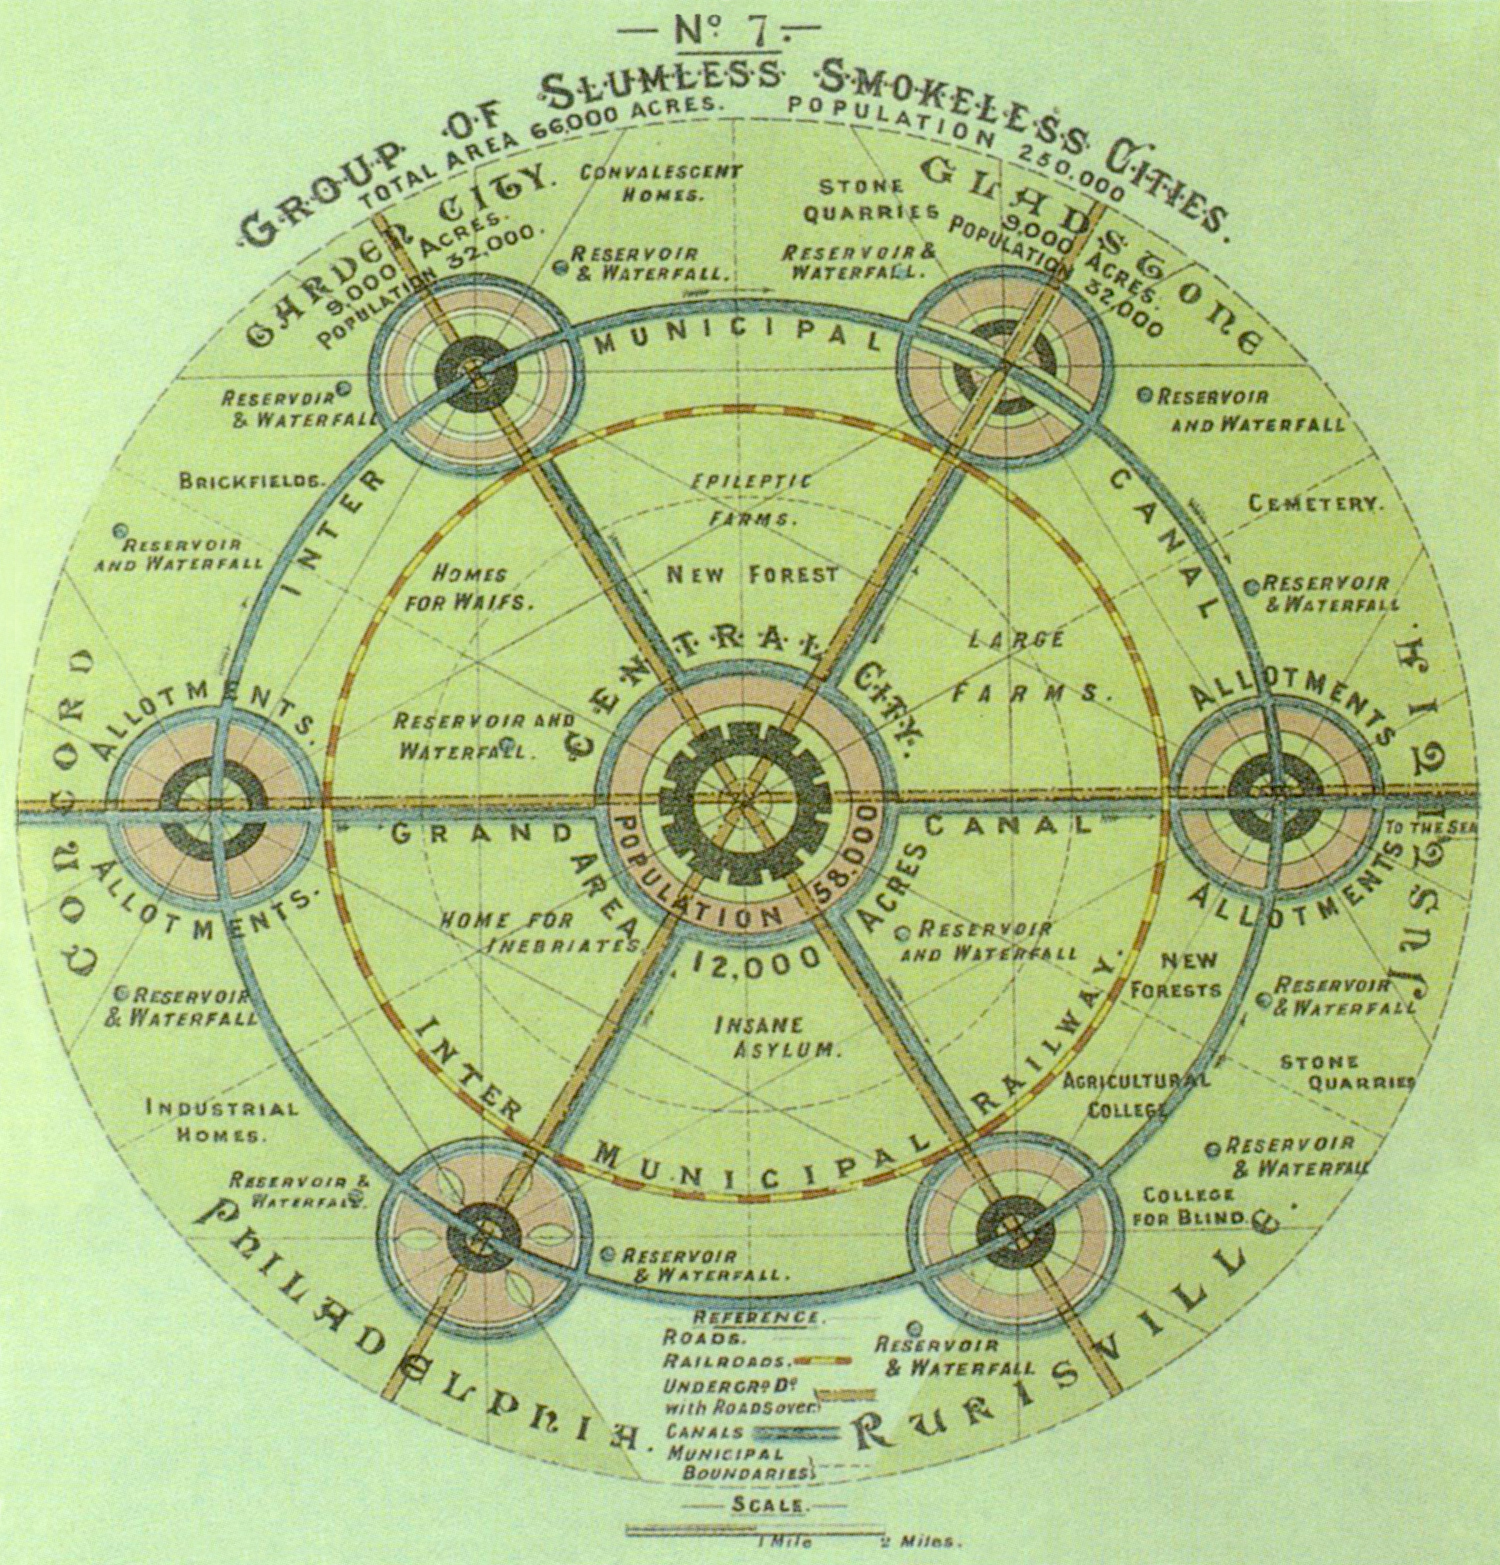
\includegraphics[width=10cm]{image_folder/GardenCityConcept_EbenezerHoward.jpg}
\caption{Konzept der Gartenstadt von Ebenezer Howard}
\label{fig:GardenCityConcept_EbenezerHoward}
\end{figure}

Interessant sind hier die "landwirtschaftlichen Gürtel" rings um die Städte und das Marktzentrum - den sogenanten "Crystal Palace" im Stadtzentrum.
Ein Ringförmiger Markt, der einem gläsernen Gewächshaus ähneln soll, das Waren aus der umliegenden Landwirtschaft direkt an den Verbraucher vertreiben kann. Generell bleibt festzuhalten, dass Howard bereits 1898 nicht nur ein Konzept zur Verankerung von Landwirtschaft innerhalb von urbanen Gebieten erdachte sondern auch Ideen entwickelte, wie die urbane Bevölkerung mit den Lebensmitteln versorgt werden kann.

Betrachtet man zum Beispiel Städte wie Boston, USA fällt auf, dass Grünflächen und Grünzüge nach dem Vorbild Howard's zwar eine wichtige Rolle in der Stadtplanung spielen, diese Grünflächen aber meist als Parks und Freizeitanlagen angelegt wurden. Dies war lange das von der Allgemeinheit als "ländlich" verstandene Bild von Natur innerhalb einer Stadt.

Der urban landwirtschaftliche Aspekt wurde aber in den darauffolgenden Jahren durch nachfolgende Stadtplaner oft übergangen. Für den folgenden Stadtwachstum verkam die Urbane Landwirtschaft zur Ausgestaltung von mühevoll angelegten und vermeintlich natürlichen Ziergärten, die Grünflächen und Erholungsgebiete in die Städte bringen sollten. So bleibt die Frage wie es zu dieser gegensätzlichen Entwicklung kam.

In Deutschland zeigt die Sozialgeschichte das 1800 Großteile der Bevölkerung auf dem Land leben und aus der sogenannten unterbäuerlichen Schicht bestehen. Zu diesem Zeitpunkt gab es in Deutschland lediglich drei Großstädte. 1835 Endstand dann allmählich das Eisenbahnnetz welches maßgeblich zur Ausbreitung der Industrialisierung beitrug. Durch das Eisenbahnnetz konnten Arbeiter zu Ihren Arbeitsstätten pendeln, welche sich durch das wachsende Netz stärker ausbreiten konnten. Zudem konnten Güter verstärkt kostengünstig transportiert werden. Dies führte in den folgenden Jahren zum Wachstum der städtischen und ländlichen Gebiete und trug zudem zum Bevölkerungswachstum bei. 1850 bildete sich die industrielle Gesellschaft heraus und Deutschland umfasste bereits 35 Millionen Einwohner, welches damit als eines der größten Länder Europas zu dieser Zeit galt. Das enorme Städtewachstum wiederum ging auf die Binnenwanderungen, den Wachstum der Bevölkerung, Gebietserweiterungen und Eingemeindungen zurück. 1900 besaß Deutschland dann bereits 33 Städte mit mehr als 100 Tsd. Einwohnern. Der Ausbau des Schienennetzes ist dabei nicht der einzige Faktor oder gar der Grund der Industrialierung oder des Bevölkerungswachstums, dennoch trug es massiv zur Ausbreitung der Bevölkerung bei. Heinrich Heine einer der bedeutendsten deutschen Schriftsteller schrieb einmal „Welche Veränderungen müssen jetzt eintreten in unserer Anschauungsweise und in unsern Vorstellungen! Sogar die Elementarbegriffe von Zeit und Raum sind schwankend geworden. Durch die Eisenbahnen wird der Raum getötet, und es bleibt nur noch die Zeit übrig“. Dabei bot die Bahn natürlich nicht nur Vorteile. Sie trug maßgeblich zur Veränderung des Landschaftsbildes bei und brachte Rus und Lärm in die Landschaften und Städte. Durch wachsende Infrastrukturen und der Industrie aber verdichteten sich im laufe der 20. Jahrhunderts die urbanen Gebiete.

Lieberecht Migge schrieb 1926 in Hinblick auf diese Entwicklung "Das grüne Manifest" in dem er das "Leiden" der Städte zum Teil auf die Industrialisierung zurück führt. Er bezeichnet das "Land" (hier der ländlich rurale Freiraum) als Frischluftbehälter und als universale Erweiterungszone. Interessant ist hier auch dass er das "Land" nicht nur als physischen Freiraum sondern auch als Freiraum für den Geist des Menschen betrachtet in dem er seine Identität frei entfalten und entwickeln kann. Parolen ähnliche Leitsätze wie "Schafft Stadtland" oder "Die Städte sollten Ihr eigenes Land umarmen" implizieren die Grundidee des ruralen Raumes innerhalb der Stadtgebiete. "Man Pflanze!" heißt es weiter. Aber das Gepflanzte soll auch Mehrwert erfüllen, keine einfachen nach Blumenbeet anmutenden Grünflächen um der Optik willen, sondern Parkanlagen, Spielplätze und Bäder, die der Allgemeinheit einen Mehrwert bieten. Aber auch Gedanken zur Selbstversorgung kommen auf. So schreibt er Beispielsweise von Nutzgärten mit einer größe von 80qm pro Einwohner auf denen Nahrungsmittel für den Eigenbedarf angebaut werden sollten. Was sich zunächst nach einer Wunschvorstellung anhört, könnte in Ausnahmesituationen Leben retten. Nach dem zweiten Weltkrieg litten beispielsweise viele Stadtbewohner an Nahrungsmangel. In der Nachkriegszeit änderte sich daher der Blick auf Urbane Landwirtschaft massiv. In städtischen Hinterhöfen wurden zum Beispiel auch Kartoffeln und Rüben angebaut. Erholungsparks und Spielplätze wurden in Nutzgärten gewandelt da reine Grünplätze mehr und mehr als unwirtschaftlich betrachtet wurden. Migge war sich dessen bewusst und versuchte in seinem Manifesto eine Art Richtlinie für den Städtebau zu entwickelten. So verurteilt er auch den Wohnraum einzelner Menschen über deren Bedarf hinweg und fordert ein verstärtkes Bewusstsein für Müll und Nahrungsmittel. Die Städter sollten in einer Art Gleichgewicht mit dem Land leben das betont er wei folgt: "Die Stadt muss auch geben dem Land - will sie leben vom Land". Eine der wichtigsten Architektonischen Eigenschaften von Städten, das Bauen von Wohneinheiten übereinander, verurteilt er und bezeichnet das "übereinander" als die Wurzel allen übels. Dies ist zwar eine äußerst radikale Ansicht, repräsentiert aber den Wunsch nach freier Entfaltung und individualität des Wohnraumes. Er wünschte sich weiter ein neues Dasein im ländlich urbanen Raum welches durch harte Arbeit, Bescheidenheit und Naturverbundenheit geprägt sein sollte.

Zusammen mit Howard und Migge erdachten viele Gelehrten intelligente Stadtkonzepte so auch Ernst May der 1922/23 Trabantenstädte erdachte, die von "Kulturbändern" umgeben sein sollten, auf diesen dann eine intensive Landwirtschaft entstehen sollte. Gemüse und Kleinvieh von Kleinbauern sollte so herangezogen und -gezüchtet werden, welches dann als Nahrungsmittel für die Siedlungen gefördert werden sollte. Dieser Ansatz floss in den 1920er Jahren in den Städtebau mit ein und stärkte dabei das Kleingartenwesen.

Mitt der 1970er Jahre erreichte dann die Iddee der Community Gardens Europa. Hier nutzten fleißige Anwohner benachteiligter Viertel, beispielweise in New York, Brachflächen der Stadt und pflanzten Blumen, Gemüse und Kräuter an. Diese Bewegung erreichte Deutschland etwa 1990. Berlin gilt heute als eine der deutschen Hochburgen für Gemeinschaftsgärten. Zusammenfassend lässt sich sagen, dass urbane Landwirtschaft häufig als Rettungsring betrachtet wird. Das Bewusstsein für die vermeintlich lebensrettende Methode der Landwirtschaft scheint immer dann stark zu wachsen wenn es den Bewohnern urbaner Gebiete besonders schlecht ergeht. Dies wurde auch 2007 deutlich als schwere Waldbrände in Griechenland wüteten. Die Krise führte zu einem vermehrten Anbau von Nahrungsmitteln innerhalb der griechischen Städte und führte sogar zur Ausbeutung von städtisch landwirtschaftlichen Räumen durch Zivilisten. Seit 2012 wird die urbane Landwirtschaft von der Zivilgesellschaft oder den einzelnen Gemeinden verbreitet.

Ein weiteres Beispiel für den Antrieb von Urbaner Landwirtschaft in Kriesenzeiten lieferte Kuba in den 90er Jahren. Durch den Zusammenbruch der Sowjetunion kam es auf der Insel auch zum Zusammenbruch der dortigen Wirtschaft, da diese stark von der sowjetischen Ölversorgung abhing. Durch den fehlenden Rohstoff konnten beispielsweise keine Erntemaschinen betankt werden. Zudem mangelte es auch an Düngern und Pestiziden. Die Einwohner der Insel setzten immer stärker auf die urbanen Anbaumethoden. Heute gehört der Inselstaat zu den Ländern die große Fortschritte zur Bekämpfung von Hunger durch Urbane Landwirtschaft gemacht haben.

Detroit welche von einer starken Wirtschaft profitierte geriet vor Jahrzehnten in eine schwere Krise. Die einstige florierende Automobilbranche liegt brach. Dadurch zogen viele arbeitslose Einwohner aus der Stadt. Durch die ungenutzten urbanen Gebiete konnte aber in den darauffolgenden Jahren eine aufsteigende Landwirtschaft entstehen. Brachland und Dachterrassen wurden nun zu ca. 1200 fruchtbare Gärten verwandelt. „Nach einer Studie der Michigan State University könnte Detroit mit Stadtfarmen, Nachbarschaftsgärten und Gewächshäusern drei Viertel ihres Gemüses und vierzig Prozent ihres Obstes selbst produzieren.“ https://www.bzfe.de/inhalt/gemuese-statt-cadillac-urban-gardening-in-detroit-27424.html

Urbane Landwirtschaft heute

Die Urbane Landwirtschaft hat es mittlerweile immer öfter in die öffentlichen Medien geschafft. Durch die Ansätze des Guerilla Gardenings oder Skyfarmings erzeugt das Themenfeld auch größeres Interesse, beinhaltet aber auch Projekte und Ansätze ohne deutlichen Mehrwert. Dies bedeutet das manche Methoden der UL einen unzureichend Nachhaltigen Aspekt bieten oder schlichtweg nicht wirtschaftlich arbeiten. Beispiele für UL folgen in Kapitel X. Es kommt hinzu dass die UL keine nennenswerte Rolle in der Ausbildung von Landwirtschaftsberufen spielt. Das Bewusstsein für die moderne Stadt ändert sich durch ambitionierte Architekten, Stadtplaner und Einwohner dennoch stetig und Brachflächen innerhalb von Städten werden nicht mehr nur einfach begrünt sondern nehmen auch einen immer größeren Platz in der Planung ein. 

"Man versucht die Landwirtschaft als Partner zu gewinnen, um die Freiflächen in der Stadtregion zu unterhalten und als öffentlichen Raum zu bespielen." Frank Lohrberg - Urban Gardening Christa Müller

\subsection{Aspekt der Romantik und Landlust in Bezug auf Urbaner Landwirtschaft am Beispiel Deutschland}

Eine romantische Vorstellung des Landlebens und der Landwirtschaft bei der Begrünung von Städten ist ein weit verbreitetes Phänomen und dazu nicht neu. Wie zuvor beschrieben trat dieses Phänomen in der Vergangenheit häufiger auf. Da Landwirtschaft bis zur Phase der Industrialisierung auch in der Stadt oder im städtischen Umland stattfand und die Versorgung so durch eigens angebaute Lebensmittel in der Subsitenzwirtschaft bewerkstelligt wurde, bildet diese "ursprüngliche" Form der Landwirtschaft in Deutschland und auch global gesehen die Tradition der Nahrungsmittelversorgung ab. Erst mit der Verdichtung der Städte und der Umwandlung von einer Agrar- zur Industriegesellschafft verschwanden die städtischen Gärten und Landwirtschaftsflächen. Dieser Gesellschaftsumschwung führte dann zur Urbanisierung.

Enge Wohnverhältnisse und 

Die "Landlust" in Deutschland, welche in der folgenden Arbeit durch das Verlangen nach einem natürlichen ländlichen Lebensstil definiert wird, äußerte sich dann zum Beispiel im Urban Gardening, im Konzept der Gartenstadt-, die Siedlungs- und die Kommunenbewegung sowie im Kleingartenwesen. Diese Bewegungen sollten einen Gegensatz zur Industriewirtschaft und der damaligen Politik vom letzten drittel des 19. Jahrhunderts bis zum ersten Weltkrieg bilden.


\subsection{Heutige und zukünftige globale Landnutzung}


Das Umdenken der allgemeinen Gesellschaft fandt dennoch erst zunehmend nach dem ersten Weltkrieg statt. Zuvor 



\section{Gegenwart der urbanen Landwirtschaft}
\subsection{Motivation der urbanen Landwirtschaft}

\subsection{Aktueller Stand der urbanen Landwirtschaft}

Wie gut ein Land versorgt ist hängt von vielen Faktoren ab. Darunter zählt der wirtschaftliche Status, die Verfügbarkeit von Ressourcen, die jeweilige Ernährungspolitik und wie gut die Infrastruktur zur Lebensmittelversorgung (Transport, Lager, Vermarktung uvm.) ist. Demnach unterscheiden sich die Aufgaben der urbanen Landwirtschaft einer Stadt im besonderen je nach dem „Entwicklungsgrad“ des Landes \footcite{SmitUrbanToday}. In Entwicklungsländern dient sie vorwiegend der Subsistenz der Stadtbewohner und als zusätzliches Einkommen \footcites[vgl.][S.70]{Nugent2000TheEconomies}[S.26f]{SmitUrbanToday}. In Industrieländern hingegen ist sie mehr von sozialpolitischer Natur \footcites[vgl.][S. 21]{Berges2004UrbaneStadt}[S.26f]{SmitUrbanToday}. Moustiers Untersuchungen fasst die Gründe für die urbane Landnutzung in Entwicklungsländern gut zusammen: Besonders oft verwendet für den städtischen Pflanzenanbau seien schnell verderbliche Lebensmittel wie Blattgemüse oder Tomaten. Durch den Anbau nahe der Stadt wird der Transportweg verkürzt und die Produkte gelangen in kürzester Zeit zum Konsumenten. Zusätzlich ist in den meisten Fällen die Lieferkette kürzer, was den Preis der Lebensmittel senkt. Bei weniger verderblichen Lebensmitteln schwanke der Anbau zwischen den Stadtrandgebieten und ruralem Anbau. Den Konsumenten sei auch die Frische der Produkte besonders wichtig, da ihnen oft eine geeignete Lagerung wie Kühlschränke fehle. Bedenklich sei die Qualität der Lebensmittel im Hinblick auf die verunreinigte Wasser- und Bodenqualität sowohl in der Stadt als auch im Umland. Jedoch sorge die Nähe für einen besseren Informationsaustausch zum Anbau. Das erleichtert den städtischen Gemeinden die Kontrolle ihrer Ernährungssicherheit. Darüber hinaus habe die dortige urbane Landwirtschaft oft damit zu tun, dass viele Städte geschichtlich an rohstoffreichen Gegenden angesiedelt waren und das Umland von Städten daher gute Anbaubedingungen vorweist. Die saisonalen Bedingungen spielen hier ebenfalls eine wichtige Rolle. In „schlechten“ Jahreszeiten sind Stadtbewohner angewiesen auf die Zufuhr von ferner angebauten Nahrungsmitteln. Die Datenerhebungen von Zezza et. al. zur urbanen Landwirtschaft in Schwellen- und Entwicklungsländern zeigt den Zusammenhang zwischen der Einkommensstärke der Stadtbewohner und der Beteiligung an urbaner Landwirtschaft:
\begin{displayquote}
„With very few exceptions, a clear negative correlation between participation in agricultural activities and level of welfare is noted. Participation rates for the poorest quintile are extremely high, over 50\% in 8 out of 15 countries, proving how urban agriculture plays an important role for a non-negligible number of poor households in the developing world.“\footcite[S.268]{Zezza2010UrbanCountries}
\end{displayquote}
UL in Industriestaaten sei hingegen nicht so essentiell wie in Entwicklungsländern. Smit et. al. geben dafür drei Gründe an: Zum einen sei das Verhältnis zwischen den Lebensmittelkosten und dem urbanen Haushaltsbudget in Industrieländern geringer. Während Stadtbewohner im globalen Norden ein Drittel bis ein Fünftel ihres Haushaltsbudgets für Essen verbrauchen, liegt der Anteil der Lebensmittelkosten in ärmeren Ländern zwischen ein Drittel und vier Fünftel. Ein weiterer Grund sei, dass die Infrastruktur zur Nahrungsmittelversorgung vollständiger sei. Und der dritte Punkt ist, dass Lebensmittel sowohl eine höhere Qualität haben als auch zugänglicher seien für die Stadtbevölkerung \footcites[vgl.][S.27]{SmitUrbanToday}. Ferner führte Das Leibniz-Zentrum für Agrarlandschaftsforschung 2011 bis 2014 eine Innovationsanalyse zu urbaner Landwirtschaft in den USA angewandt auf Deutschland durch. Eine der Erkenntnisse dieses Forschungsprojektes war, dass heutige UL-Formen in den USA und Deutschland vorwiegend soziale Neuerungen zeigen \footcite{Berges2004UrbaneStadt}.  






\subsection{Aktueller Stand der Lebensmittelversorgung in Städten (im Bezug auf Nachhaltigkeit)} 

"Nahrung ist eine grundlegende Basis für die Existenz menschlichen Lebens". Hiermit fasst Stierand Informationen aus von Blackenburgs Text in "Zukunft, Welternährung —Gegenwartsprobleme und Strategien" zusammen. \footcite{Stierand2008StadtLebensmittel} „Jeder Mensch benötigt eine angemessene Ernährung, um körperlich und geistig leistungsfähig zu bleiben. (Auch für die Aufrechterhaltung der Gesundheit und die Abwehr von Krankheiten ist ausreichende Ernährung wichtig.“ \footcite{Blanckenburg1987ZukunftDie}

Laut P. Stierand hat die Erzeugung und Verarbeitung von Lebensmitteln in der heutigen Zeit "ihre Bindung an die Verbrauchsräume weitgehend verloren, schnelle und gute Transportmöglichkeiten erlauben weltweiten Handel. So ist die Landwirtschaft in und um Städte nicht mehr überlebenswichtig.\footcite{Stierand2008StadtLebensmittel, S.122f}

\begin{figure}[htp]
\centering
\includegraphics[width=10cm]{image_folder/ernährungsmastabaenderung.png}}
\caption{Änderung des Ernährungsmaßstabs}
\label{fig:Änderung des Ernährungsmaßstabs}
\end{figure}

Mit der Entstehung von regionalen und nationalen Ketten dehnte sich der Handel aus und das Ernährungssystem erfuhr eine "Delokalisation“ (Montanari 1993: 188-192). Seitdem ist "die Bindung zwischen Wohnort und Nahrung [...]aufgehoben, die Ernährung ist nicht mehr von saisonalen Engpässen und Überschüssen abhängig.\footcite{Stierand2008StadtLebensmittel, S.122f}

\subsubsection {Ernährung in der Stadt}
  
Laut P. Stierand wurde der Mensch erst durch das moderne Ernährungssystem zum ausschließlichen Verbraucher von Lebensmitteln. Er begründet dies mit dem Zitat aus „Eßkultur heute: Was, wie und wo essen wir?“ In: Dr. Rainer Wild-Stiftung (Hg.): Gesunde Ernährung zwischen Natur- und Kulturwissenschaft. Münster, 41-56. von Spiekermann, Uwe (1999b):
"Wir sind Konsumenten. Wir essen nicht mehr selbstgezogene Lebensmittel, sondern wir verzehren Produkte, deren Herkunft, deren Produktion und Geschichte uns nur in Ausnahmefällen bekannt ist. Essen als Resultat einer arbeitsteiligen Nahrungskette […] wird uns fremd, zumindest aber fremder. (Spiekermann 1999b: 48)

\subsection{Formen der urbanen Landwirtschaft}
\subsection{Zusammenfassung}


\newpage
\listoffigures

\begingroup
\singlespacing
\setlength\bibitemsep{10pt}% oder was auch immer
\printbibliography
\endgroup
\end{document}
